% kuleuventheme2 by Janez Kren, September 2017, janez.kren@kuleuven.be, based on:
% kuleuventheme 1.3 by Roland Pastorino, 2013 roland.pastorino@kuleuven.be / www.rolandpastorino.com

\documentclass[11pt,t]{beamer}
\usetheme{kuleuven2}	%THEME OPTIONS for LOGO: kul (default), kulak, lrd,    ; OPTIONS for TITLE PAGE: normal (default), sedes


%%% OTHER SETTINGS
\usefonttheme[onlymath]{serif}			% math font with serifs, delete to make it sans-serif
\setbeamertemplate{footline}[body] 		% delete this line to remove footline bar on all frames
%\usepackage[orientation=landscape,size=custom,width=16,height=9,scale=0.5,debug]{beamerposter} %enable for widescreen 16:9 ratio
%\titlegraphic{ \includegraphics[width=.2\paperwidth]{mytitlepagepic.png} } %optional title page image


%%% ADDED PACKAGES:
\usepackage[dutch]{babel}
\usepackage{amsfonts}
\usepackage{amssymb}


%%% TITLE PAGE INFO:
\title[Eindpresentatie]{Semantische positietracking van een mobiele robot in ziekenhuisgangen d.m.v. visie} %[]] will appear in footline
\subtitle{Eindpresentatie}

\author{Olivier Van den Eede}
\institute{KU Leuven - De Nayer}
\date{25 Juni 2019}




\begin{document}
\csname beamer@calculateheadfoot\endcsname %recalculate head and foot dimension


 %%
 %%  0. TITLE PAGE and TABLE OF CONTENT
 %%
% Title page
\begin{frame}[plain,noframenumbering]
	\titlepage
\end{frame}
	

% Table of Contents
\begin{frame}{Inhoud}
	\hfill	{\large \parbox{.961\textwidth}{\tableofcontents[hideothersubsections]}}
\end{frame}




 %%
 %%  SECTION 1 - Probleemstelling
 %%
\section{Probleemstelling}
\begin{frame}[fragile]{Probleemstelling}
	Ziekenhuizen kampen met volgende problemen:
	\begin{itemize}
		\item Personeelstekorten
		\item Hoge werkdruk voor zorgpersoneel
	\end{itemize}

	Onder andere veroorzaakt doordat personeel verantwoordelijk is voor textiellogistiek en goederenstroom.
\end{frame}

\begin{frame}[fragile]{Mogelijke oplossing}
	\begin{itemize}
		\item Automatisatie
		\begin{itemize}
			\item Moeilijk door infrastructuur en bestaand logistiek materiaal.
		\end{itemize}
		\item \textbf{Autonoom Geleid Voertuig (AGV)}
		\begin{itemize}
			\item Zelfstandige navigatie doorheen ziekenhuisgangen
			\item Uitgerust met sensoren en een RGB camera
			\item Semantische kaart voor navigatie
			\begin{itemize}
				\item Kaart met aanduidingen van zichtbare objecten
				\item Afmetingen, positie en ori\"{e}ntatie van deze objecten
			\end{itemize}
		\end{itemize}
	\end{itemize}
\end{frame}

\begin{frame}[fragile]{Doel masterproef}
	\begin{itemize}
		\item Onderzoeken aanwezige visuele objecten/features in ziekenhuisgangen
		\begin{itemize}
			\item Gangen zijn zeer monotoon
			\item Weinig visuele kenmerken aanwezig
		\end{itemize}
	\end{itemize}
	\begin{figure}
		\centering
		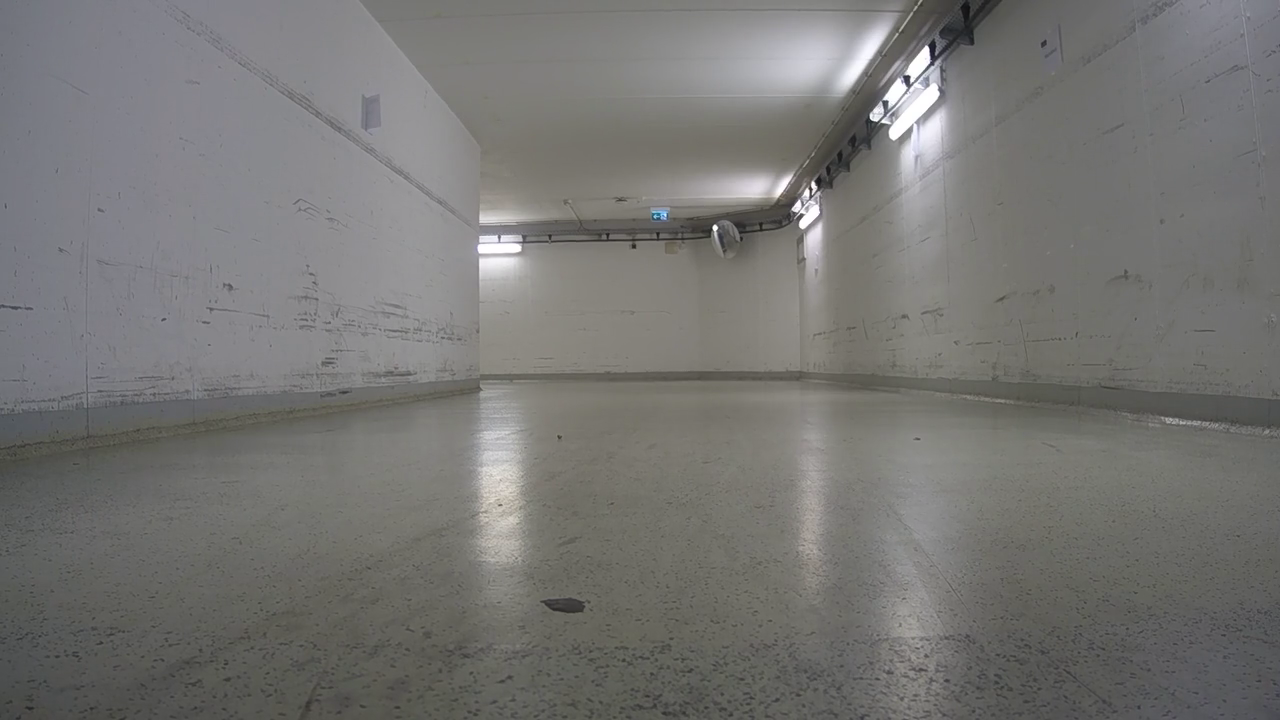
\includegraphics[width=0.8\textwidth]{graphics/gang.png}
	\end{figure}
\end{frame}
\begin{frame}{Doel masterproef}
	\begin{itemize}
		\item Zoeken naar geschikte beeldverwerkingstechnieken voor detectie van deze features
		\item Tracken van de robotpositie op basis van:
		\begin{itemize}
			\item De gedetecteerde visuele features uit 1 RGB camera
			\item De informatie op een semantische kaart
		\end{itemize}
	\end{itemize}
\end{frame}



 %%
 %%  SECTION 2 - Uitwerking
 %%
\section{Uitwerking}
\begin{frame}[fragile]{Uitwerking}
	\begin{figure}
		\centering
		\includegraphics[width=\textwidth]{graphics/pipeline1.png}
		\caption{Overzicht van het programma(1).}
	\end{figure}
\end{frame}
\begin{frame}[fragile]{Uitwerking}
	\begin{figure}
		\centering
		\includegraphics[width=0.7\textwidth]{graphics/pipeline2.png}
		\caption{Overzicht van het programma(2).}
	\end{figure}
\end{frame}

\begin{frame}[fragile]{Uitwerking}
	\begin{itemize}
		\item \textbf{Object detectie}
		\item Perspectiefpunt detectie
		\item Omgevingsrepresentatie
		\item Semantische kaart
		\item Robot positie tracking
	\end{itemize}
\end{frame}

\begin{frame}[fragile]{Object detectie}
	\begin{itemize}
		\item YOLOv2
		\begin{itemize}
			\item Veel gebruikt
			\item Single shot detectie + classificatie CNN
			\item Kan real-time werken op GPU
		\end{itemize}

		\item Datasets
		\item Annotatie beeldmateriaal
		\item Training YOLOv2
	\end{itemize}
	\begin{figure}
		\centering
		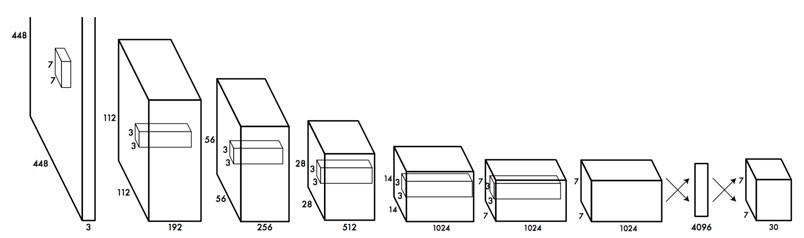
\includegraphics[width=0.7\textwidth]{graphics/yolo_cnn.jpeg}
	\end{figure}
\end{frame}

\begin{frame}[fragile]{Datasets}
	Kenmerken datasets:
	\begin{itemize}
		\item 2 video's opgenomen met RGB camera
		\item Beeldmateriaal van opeenvolgende gangen
		\item Eerste deel is validatieset, 2de deel is trainingsset
		\item 1920x1080 pixels @30Hz
		\item Herschaald naar 1280x720 pixels @15Hz
		\item 899 en 711 frames
	\end{itemize}

	Visuele kenmerken in dataset:
	\begin{itemize}
		\item Lampen
		\item Rookdetectoren
		\item Nooduitgang bordjes
	\end{itemize}
\end{frame}

\begin{frame}{Annotatie beeldmateriaal}
	\begin{itemize}
		\item Bounding-box met class label
		\item Nodig voor training van CNN
		\item Manuele annotatie d.m.v. CVAT
		\item Conversie CVAT XML-formaat naar YOLO-formaat
	\end{itemize}

	\begin{table}
		\tiny
		\caption{Annotaties in training en validatie set}
		\begin{tabular}{l | l | l | l | l | l | l}
			& Aantal frames & Rookmelder & Deurklink & Pictogram & TL-lamp & Totaal \\ \hline
			Trainingsset & 899 & 1016 & 147 & 340 & 5260 & 6763 \\
			Validatieset & 711 & 1130 & 180 & 408 & 992 & 2710 \\
		\end{tabular}
	\end{table}
\end{frame}

\begin{frame}[fragile]{Training YOLOv2}
	Aanpassen YOLOv2 hyperparameters:
	\begin{itemize}
		\item 4 detectieklassen
		\item Batch size van 64
		\item Learning rate van 0.0001
		\item Maximum van 45000 batches
	\end{itemize}
\end{frame}

%
% Perspectiefpunt detectie
%
\begin{frame}[fragile]{Uitwerking}
	\begin{itemize}
		\item Object detectie
		\item \textbf{Perspectiefpunt detectie}
		\item Omgevingsrepresentatie
		\item Semantische kaart
		\item Robot positie tracking
	\end{itemize}
\end{frame}

\begin{frame}[fragile]{Perspectiefpunt detectie}
	Perspectiefpunt nodig in volgende stap van de pipeline om hoeken tot de optische as te berekenen. Het punt kan gedetecteerd worden d.m.v. 3 verschillende methoden:
	\begin{itemize}
		\item Hoogste vloerpixel segmentatie
		\item Vloerlijn kruising
		\item Perspectieflijn kruising
	\end{itemize}
\end{frame}

\begin{frame}[fragile]{Hoogste vloerpixel segmentatie}
	\begin{itemize}
		\item ResNet segmentatienetwerk
		\begin{itemize}
			\item Elke pixel krijgt label
			\item Enkel vloerpixels worden gebruikt
		\end{itemize}
		
		\item In theorie is hoogste vloerpixel perspectiefpunt
		\begin{itemize}
			\item Fouten in segmentatieoutput be\"{i}nvloeden hoogste pixel
		\end{itemize}
	\end{itemize}
\end{frame}

\begin{frame}[fragile]{Hoogste vloerpixel segmentatie}
	\begin{figure}
		\centering
		\tiny
		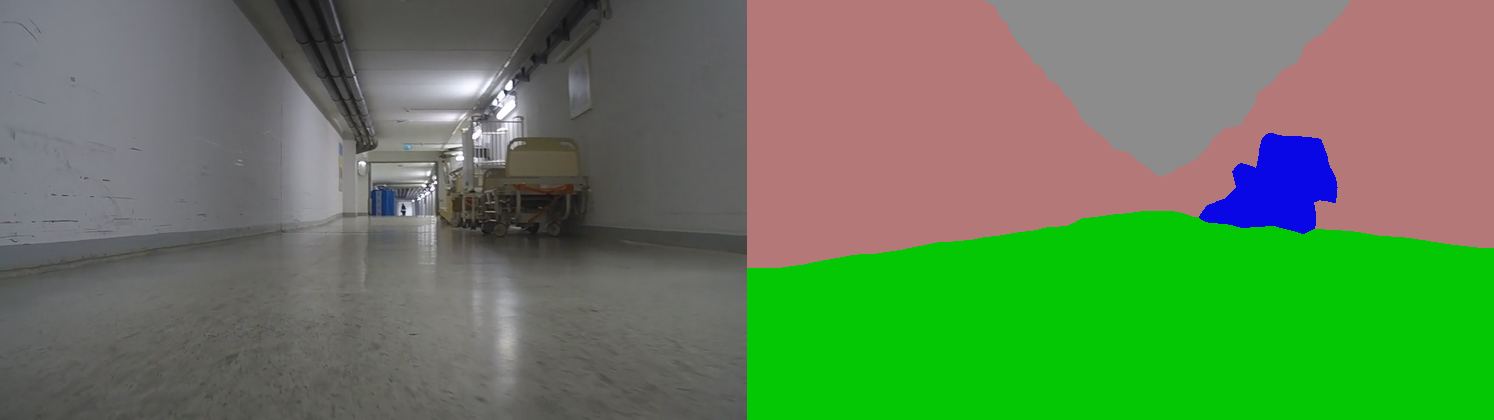
\includegraphics[width=0.9\textwidth]{graphics/segmentatie.png}
	\end{figure}
	\begin{figure}
		\centering
		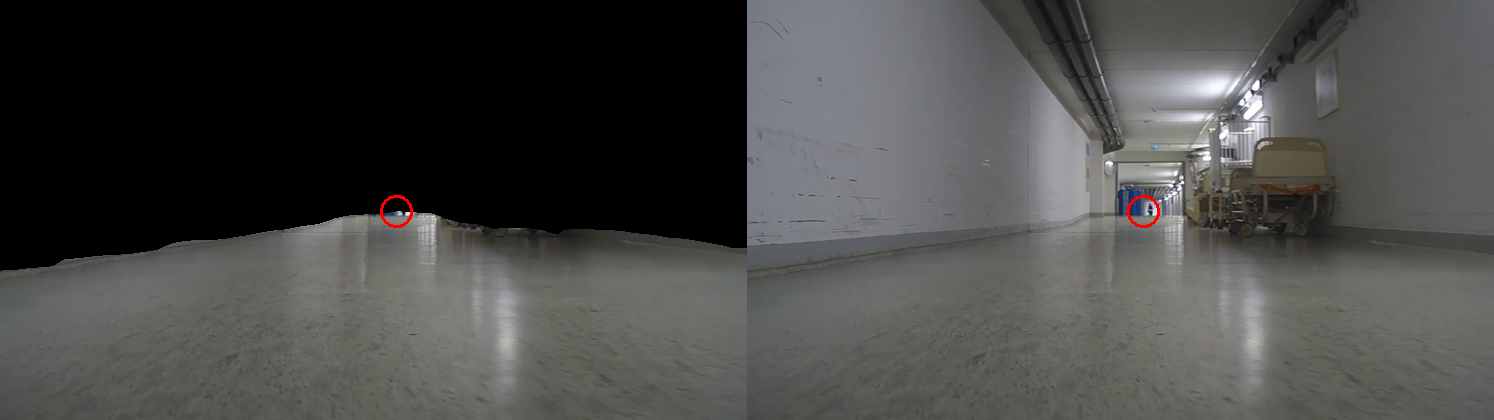
\includegraphics[width=0.9\textwidth]{graphics/seg_highest.png}
	\end{figure}
\end{frame}

\begin{frame}[fragile]{Vloerlijn kruising}
	\begin{itemize}
		\item ResNet segmentatienetwerk
		\item Edge detectie op masker van vloerpixels
		\item Zoeken van perspectieflijnen d.m.v. de Hough-transformatie op masker
		\item Kruising van perspectieflijnen is perspectiefpunt
		\begin{itemize}
			\item Dezelfde lijnen filteren op basis van de richtingsco\"{e}ffici\"{e}nt.
			\item Ideaal als 1 lijn langs elke kant van de vloer
		\end{itemize}
		
		\item Probleem:
		\begin{itemize}
			\item Vloer volgt niet de perspectieflijnen door obstructies
		\end{itemize}
		
	\end{itemize}
\end{frame}

\begin{frame}[fragile]{Vloerlijn kruising}
	\begin{figure}
		\centering
		\tiny
		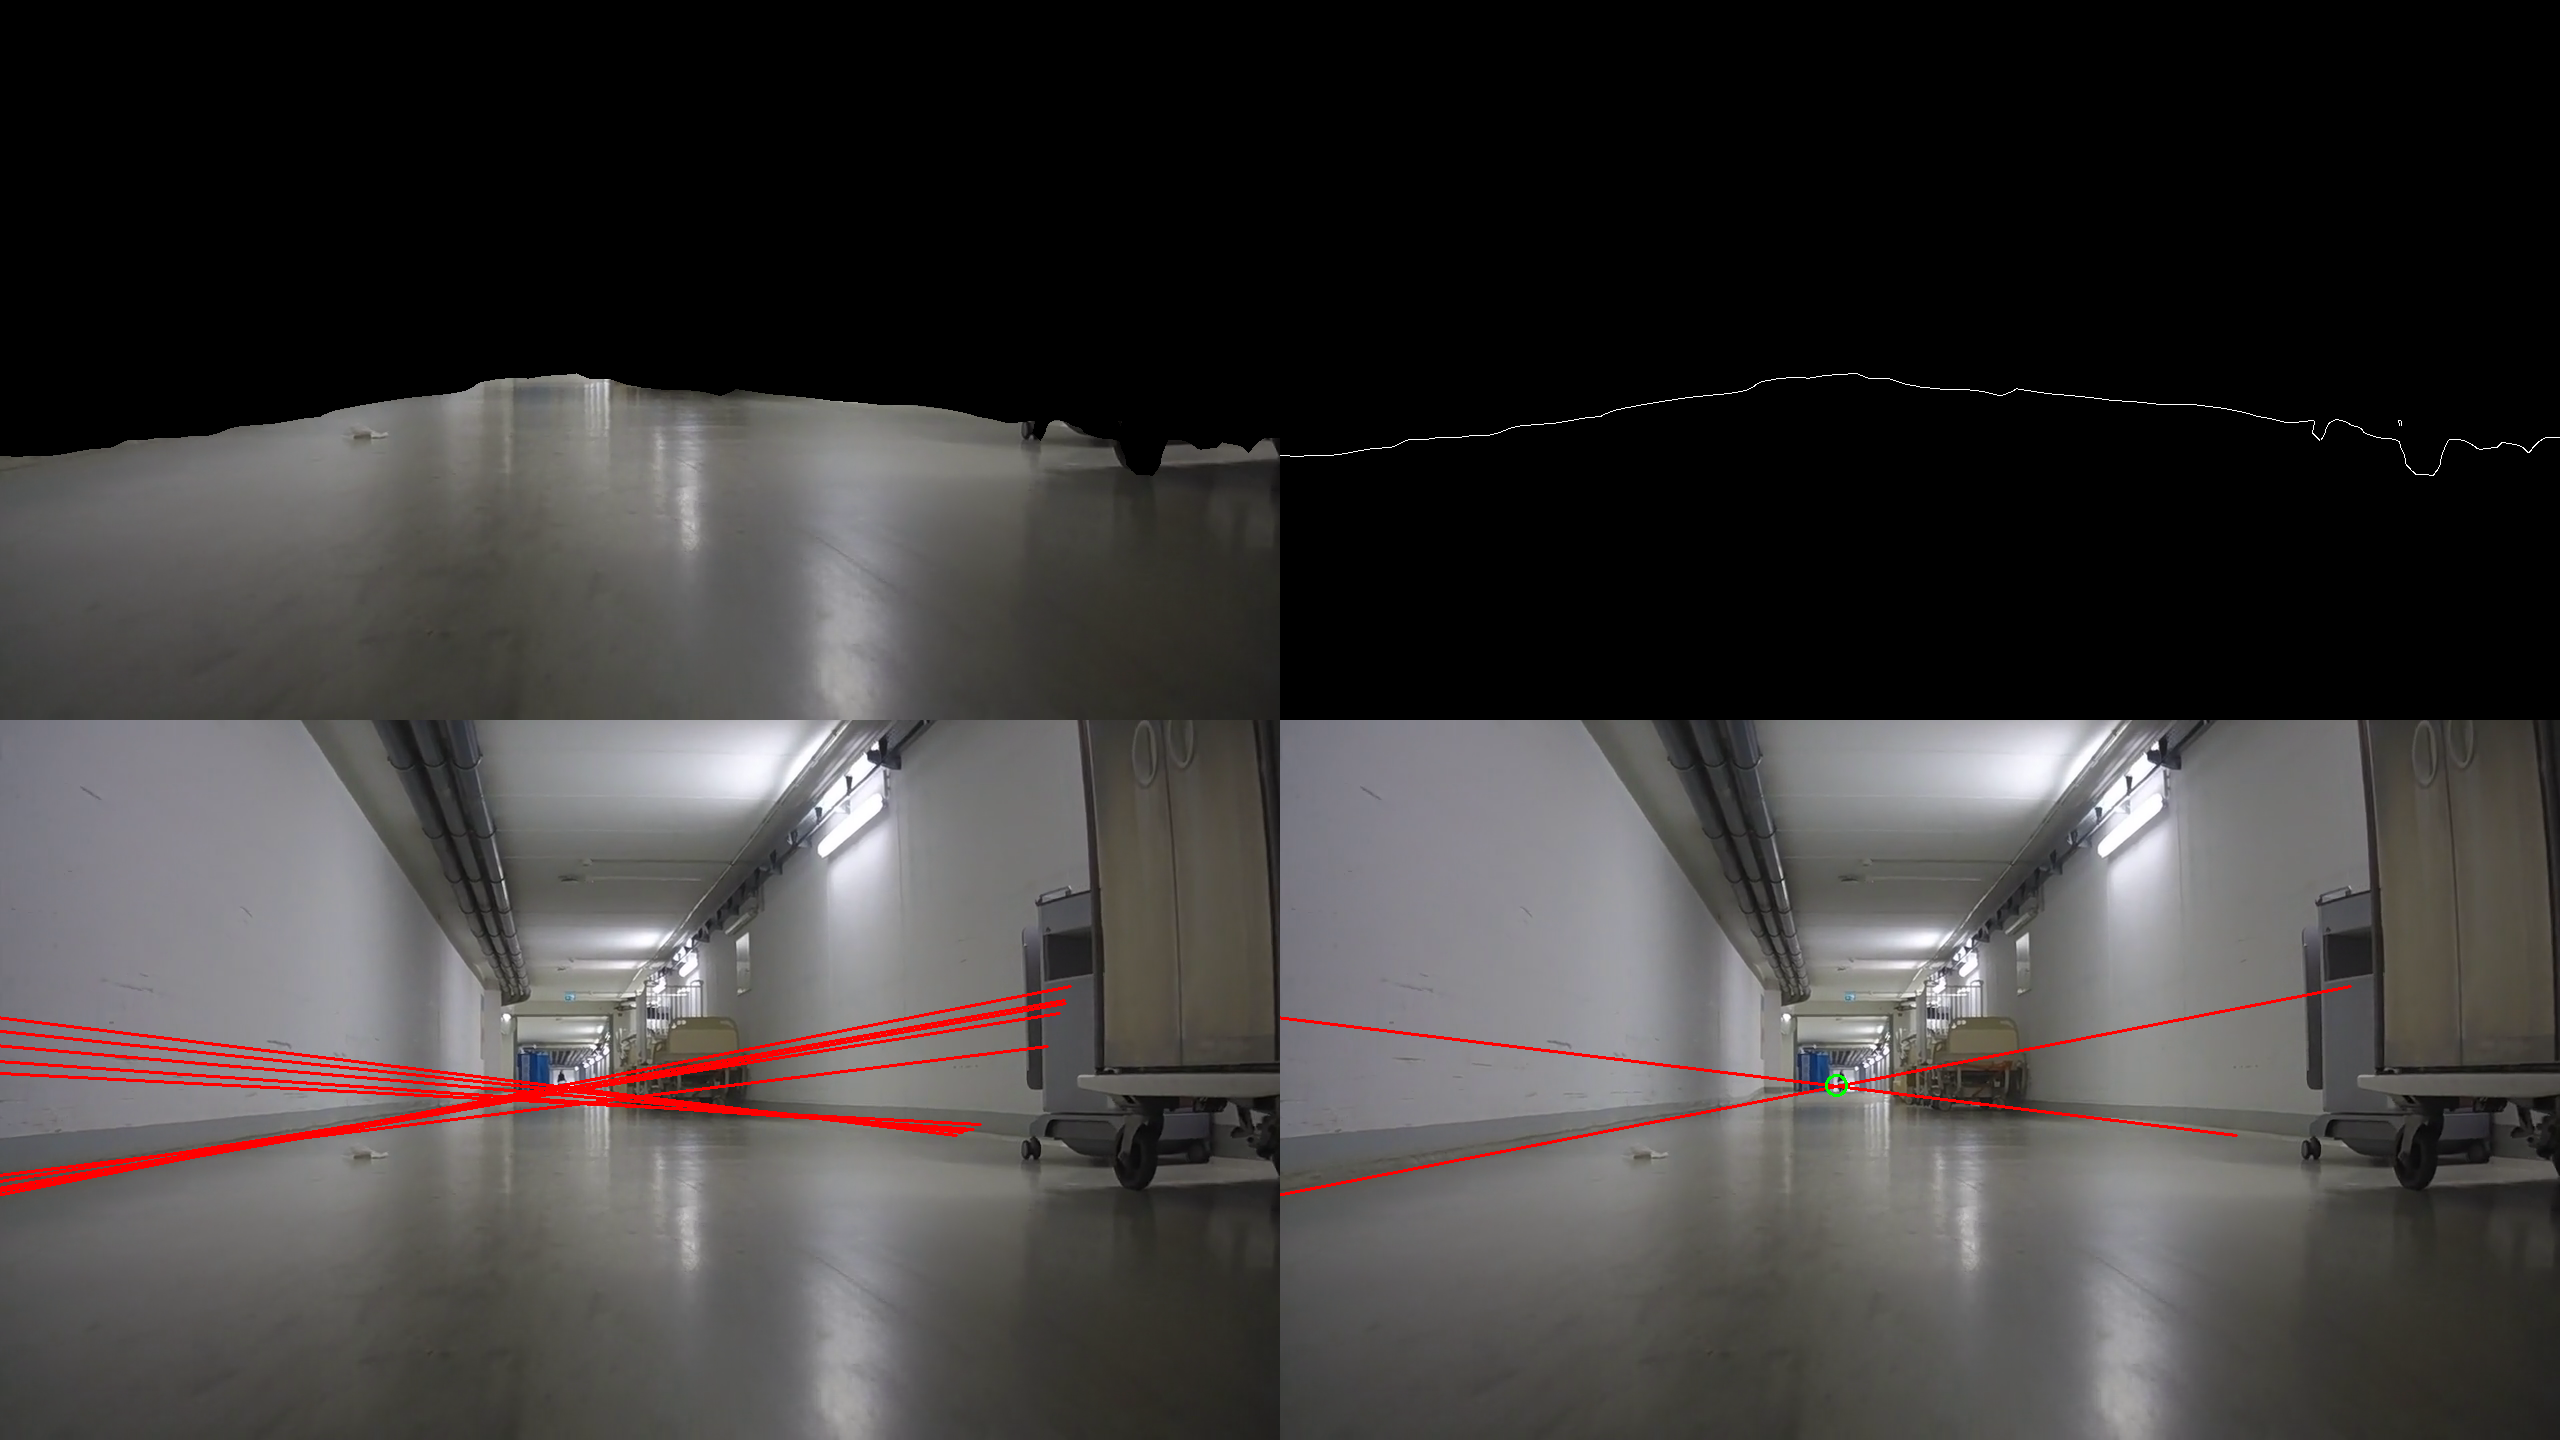
\includegraphics[width=\textwidth]{graphics/hough_floor.png}
	\end{figure}
\end{frame}

\begin{frame}[fragile]{Perspectieflijn kruising}
	\begin{itemize}
		\item Geen vloersegmentatie
		\item Canny-edgedetectie op hele grijswaardeafbeelding
		\item Variabele treshold op basis van de grijswaardemediaan. 
		\item Hough-transformatie om perspectieflijnen te vinden
		\item Filtering van horizontale en verticale lijnen
		\item Kruispunt van rechten is perspectiefpunt
	\end{itemize}

	\begin{figure}
		\centering
		\tiny
		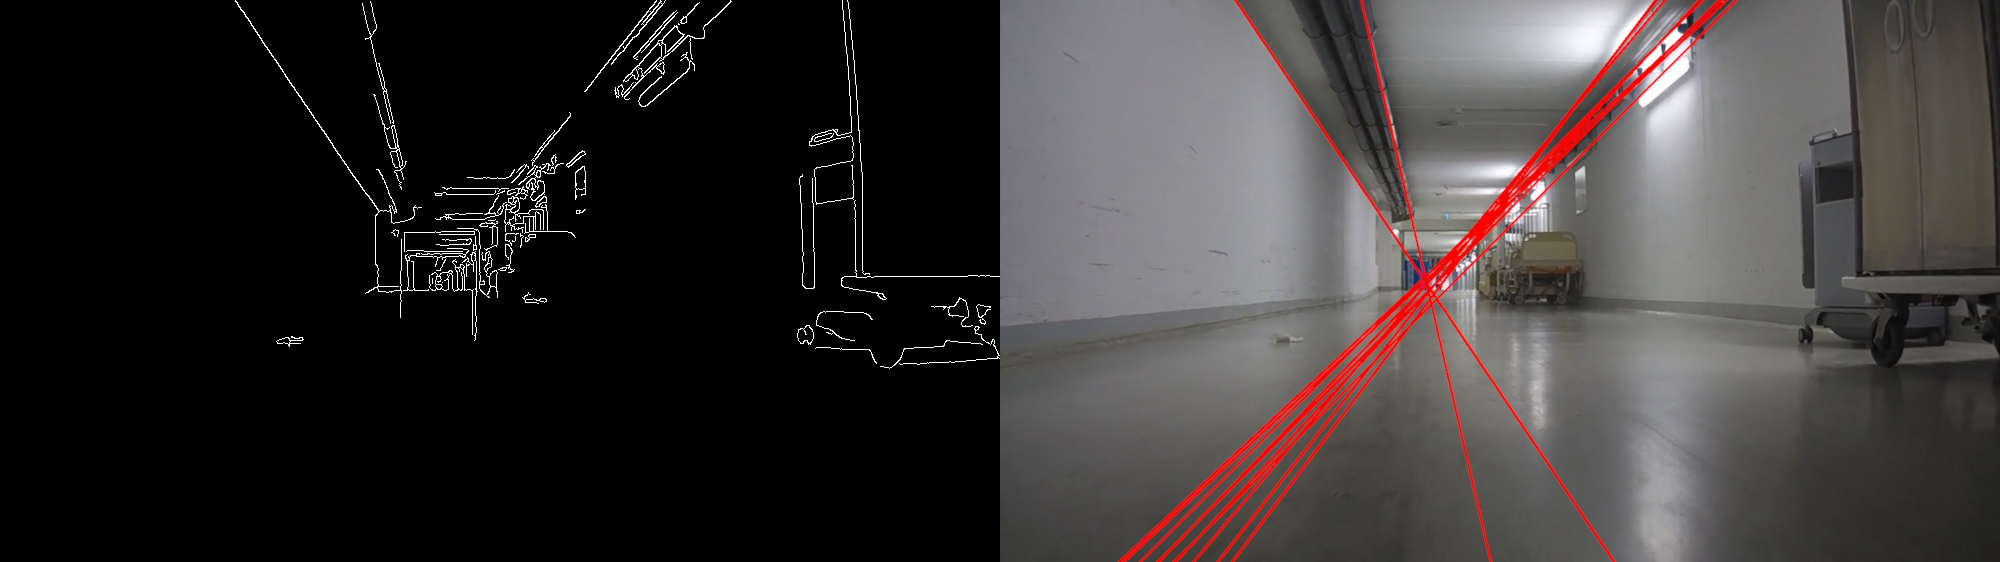
\includegraphics[width=\textwidth]{graphics/hough_all.png}
	\end{figure}
\end{frame}

%
% Omgevingsrepresentatie
%

\begin{frame}[fragile]{Uitwerking}
	\begin{itemize}
		\item Object detectie
		\item Perspectiefpunt detectie
		\item \textbf{Omgevingsrepresentatie}
		\item Semantische kaart
		\item Robot positie tracking
	\end{itemize}
\end{frame}

\begin{frame}[fragile]{Omgevingsrepresentatie}
	\begin{columns}[t]
		\begin{column}{.5\textwidth}
			\begin{itemize}
				\item Elk object heeft unieke locatie in ruimte en beeld
				\item Transformatie van afstand tot perspectiefpunt naar hoeken
				\item Bepaal hoek $\alpha_i$ voor elk object
			\end{itemize}

			\begin{block}{Verband tussen $x_i$ en $\alpha_i$}
				\[
					\alpha_i = \tan^{-1}(\frac{x_i}{l_f})
				\]
			\end{block}
		\end{column}
		\begin{column}{.5\textwidth}
			\begin{figure}
				\centering
				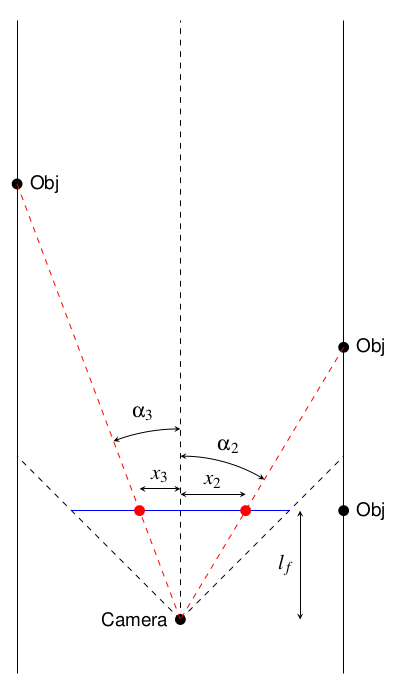
\includegraphics[height=200px]{graphics/omgeving.png}
			\end{figure}
		\end{column}
	\end{columns}	
\end{frame}

%
% Semantische kaart
%
\begin{frame}[fragile]{Uitwerking}
	\begin{itemize}
		\item Object detectie
		\item Perspectiefpunt detectie
		\item Omgevingsrepresentatie
		\item \textbf{Semantische kaart}
		\item Robot positie tracking
	\end{itemize}
\end{frame}

\begin{frame}[fragile]{Semantische kaart}
	\begin{columns}[t]
		\begin{column}{.7\textwidth}
			\begin{itemize}
				\item Representatie van alle visuele objecten binnen de ruimtes
				\item OpenStreetMap (OSM) formaat
				\item Node
				\begin{itemize}
					\item Basis OSM object
					\item Parameters in key-value formaat
					\item Object en locatie nodes
				\end{itemize}

				\item Way
				\begin{itemize}
					\item Basis OSM object
					\item Gesorteerde lijst van opeenvolgende (locatie) nodes
					\item Beschrijft een route
				\end{itemize}

				\item Inlezen via eigen parser
			\end{itemize}
		\end{column}
		\begin{column}{.3\textwidth}
			\begin{figure}
				\centering
				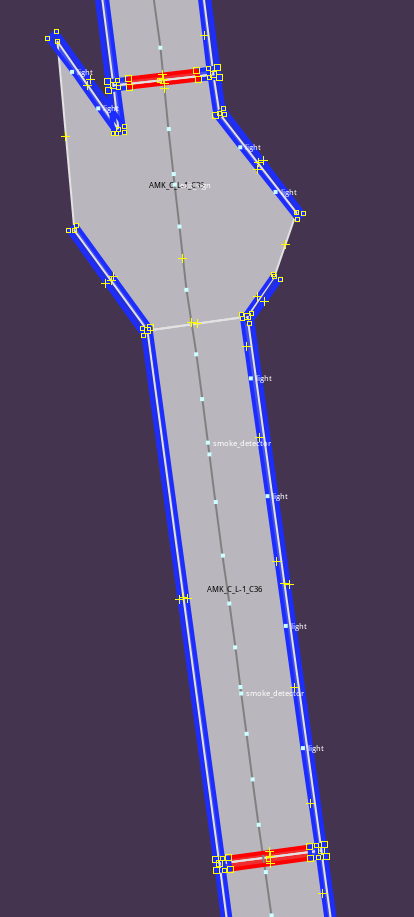
\includegraphics[height=180px]{graphics/kaart.png}
			\end{figure}
		\end{column}
	\end{columns}	
\end{frame}

%
% Robot positie tracking
%
\begin{frame}[fragile]{Uitwerking}
	\begin{itemize}
		\item Object detectie
		\item Perspectiefpunt detectie
		\item Omgevingsrepresentatie
		\item Semantische kaart
		\item \textbf{Robot positie tracking}
	\end{itemize}
\end{frame}

\begin{frame}[fragile]{Robot positie tracking}
	\begin{itemize}
		\item Corrigeer perspectiefpunt naar midden van afbeelding om rotatie van robot op te vangen
		\item Robot vertrekt op gekende locatie en volgt de gedefinieerde route vanop de kaart
		\item Robot kan niet springen en enkel vooruit rijden
		\begin{itemize}
			\item Enkel de actuele en volgende locatie-nodes worden vergeleken
		\end{itemize}
		
		\item Vergelijken Omgevingsrepresentatie en hoeken op de kaart
		\begin{itemize}
			\item Bereken score hoeveel het huidige frame lijkt op de 2 theoretische locatie-nodes
			\item Koppel gedetecteerde objecten aan objecten uit de kaart d.m.v. de hoeken
		\end{itemize}

		\item Verschillende wegingsfactoren
	\end{itemize}
\end{frame}

\begin{frame}[fragile]{Robot positie tracking}
	\begin{block}{Berekening van de score}
		\[
			score = \sum_{i=1}^{n}\big[a - |\alpha_{mi} - \alpha_{di}|\big] \cdot f_w(\alpha_{mi}) + \sum_{i=1}^{m}\big[b \cdot f_w(\alpha_{mi})\big]
		\]
		\centering
		Met $n$ het aantal gelinkte objecten, en $m$ het aantal niet gelinkte objecten. En $a$ een positieve beloningsfactor en $b$ een afstraffactor.
	\end{block}
	\begin{columns}[t]
		\begin{column}{.7\textwidth}
		\begin{block}{Berekening van de wegingsfactor}
			\[
				f_w(\alpha) = \left\{\begin{array}{lr}
					1 & \text{for } 30 < |\alpha|\\
					\frac{7\alpha + 10}{220} & \text{for } 0 \leq |\alpha| \leq 30\\
				\end{array}
				\right\}
			\]
		\end{block}
		\end{column}
		\begin{column}{.3\textwidth}
			\begin{figure}
				\centering
				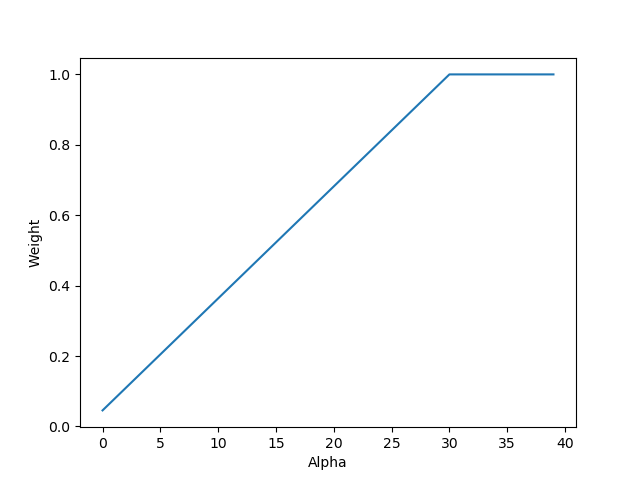
\includegraphics[width=\textwidth]{graphics/wegingsfactor.png}
			\end{figure}
		\end{column}
	\end{columns}
\end{frame}

%%
%%  SECTION 2 - Resultaten
%%
\section{Resultaten}
%
%	Object detectie
%
\begin{frame}[fragile]{Resultaten}
	\begin{itemize}
		\item \textbf{Object detectie}
		\item Perspectiefpunt detectie
		\item Lokalisatie
	\end{itemize}
\end{frame}

\begin{frame}[fragile]{Object detectie}
	\begin{itemize}
		\item Inferentietijd CPU vs GPU
		\item Invloed resolutie inputafbeeldingen
		\item Invloed aantal detectieklassen
	\end{itemize}

	\begin{figure}
		\centering
		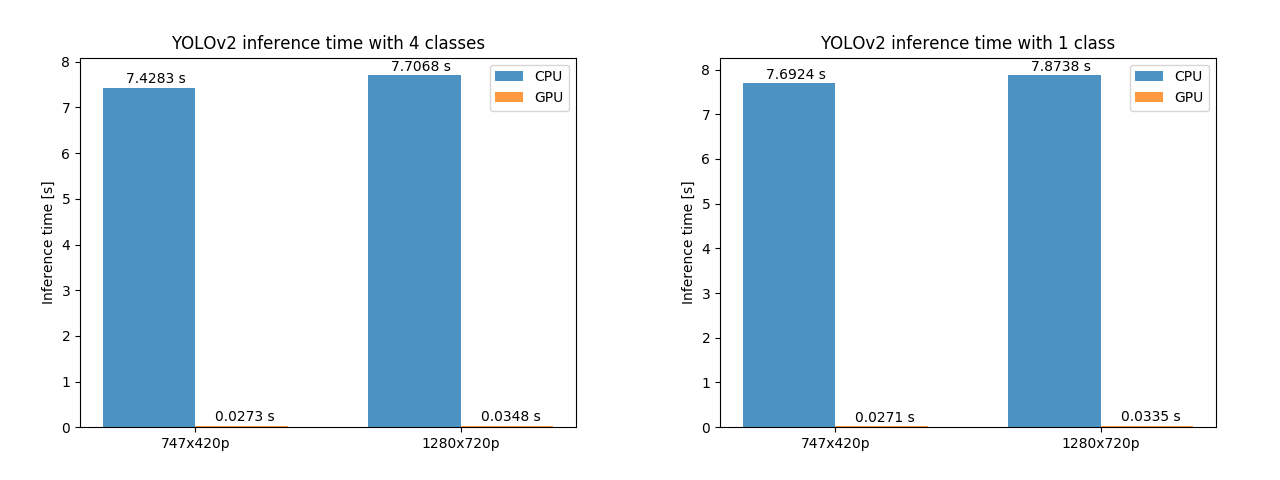
\includegraphics[width=\linewidth]{graphics/yolo_bar.png}
	\end{figure}
\end{frame}

\begin{frame}[fragile]{Object detectie}
	\begin{itemize}
		\item Nauwkeurigheid op basis van validatieset
		\item Precision-recall-curve
		\item Mean Average Precision (mAP)
	\end{itemize}

	\begin{figure}
		\centering
		\includegraphics[width=\linewidth]{graphics/yolo_pr.png}
	\end{figure}
\end{frame}

%
%	Object detectie
%
\begin{frame}[fragile]{Resultaten}
	\begin{itemize}
		\item Object detectie
		\item \textbf{Perspectiefpunt detectie}
		\item Lokalisatie
	\end{itemize}
\end{frame}

\begin{frame}[fragile]{Perspectiefpunt detectie}
	\begin{itemize}
		\item Detectietijd CPU vs GPU
		\item Vergelijking 3 detectietechnieken
		\item Invloed resolutie inputafbeeldingen
	\end{itemize}

	\begin{figure}
		\centering
		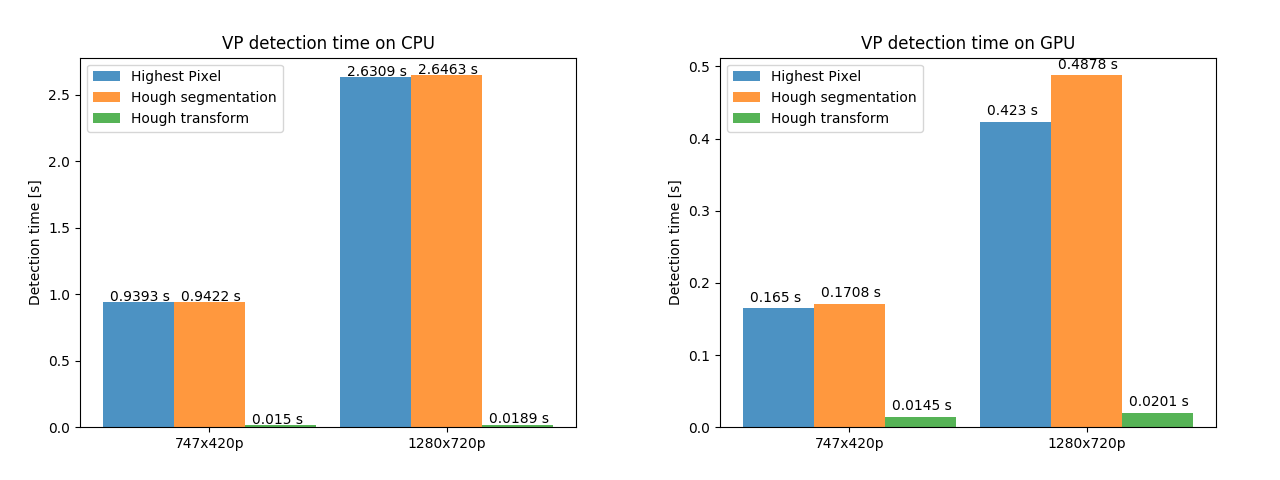
\includegraphics[width=\linewidth]{graphics/seg_speed.png}
	\end{figure}
\end{frame}

\begin{frame}[fragile]{Perspectiefpunt detectie}
	\begin{itemize}
		\item Nauwkeurigheid van 3 technieken
		\item Vergelijking met manuele annotatie van perspectiefpunt voor 100 frames
	\end{itemize}

	\begin{figure}
		\centering
		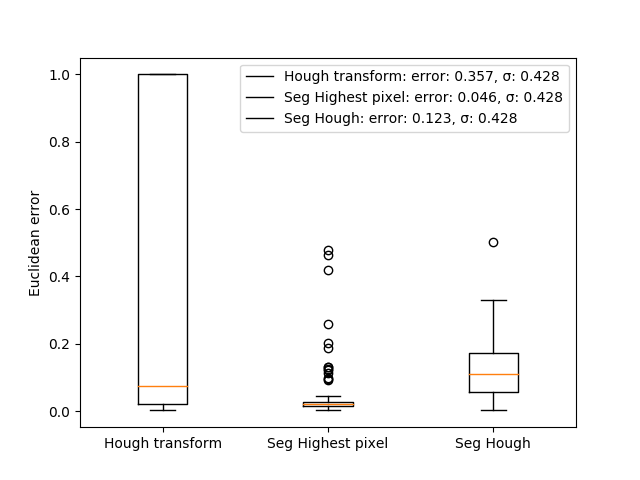
\includegraphics[width=0.6\linewidth]{graphics/seg_accuracy.png}
	\end{figure}
\end{frame}


%
%	Lokalisatie
%
\begin{frame}[fragile]{Resultaten}
	\begin{itemize}
		\item Object detectie
		\item Perspectiefpunt detectie
		\item \textbf{Lokalisatie}
	\end{itemize}
\end{frame}

\begin{frame}[fragile]{Lokalisatie}
	\begin{itemize}
		\item Iteratietijd per frame
		\item Verschil tussen perspectiefpuntdetectie met of zonder segmentatie
		\item Gemiddelde rekentijd hoog t.o.v. vorige resultaten
	\end{itemize}

	\begin{figure}
		\centering
		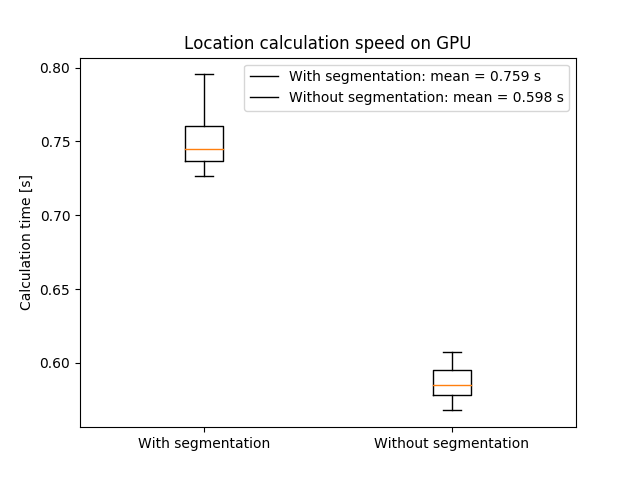
\includegraphics[width=0.6\linewidth]{graphics/loc_speed.png}
	\end{figure}
\end{frame}

\begin{frame}[fragile]{Lokalisatie}
	\begin{itemize}
		\item Profilering van de implementatie
		\item Visualisatie van kaart neemt meeste tijd in beslag
	\end{itemize}

	\begin{figure}
		\centering
		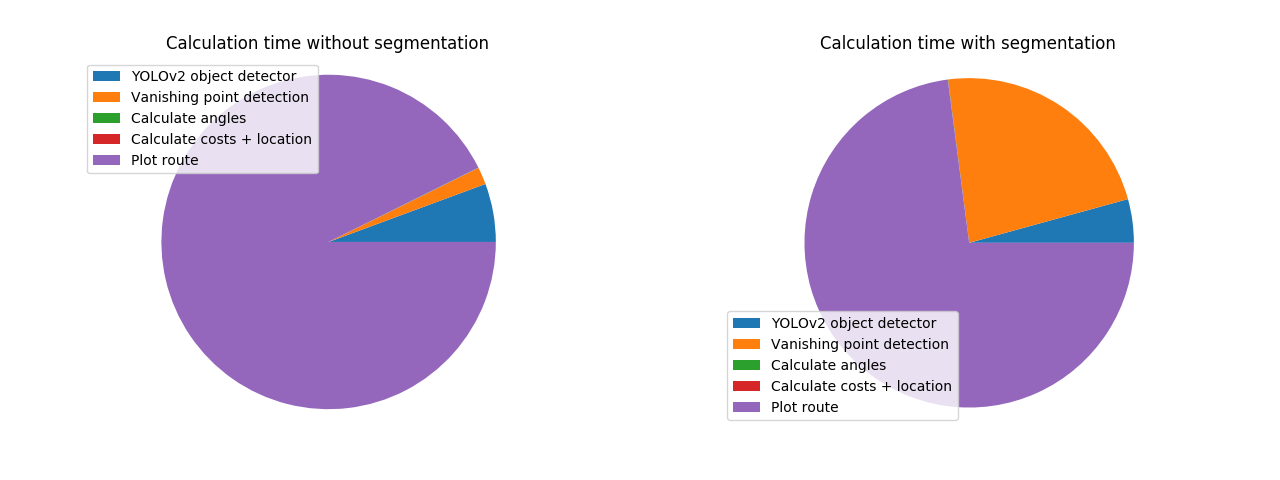
\includegraphics[width=\linewidth]{graphics/loc_time.png}
	\end{figure}
\end{frame}


\begin{frame}[fragile]{Lokalisatie}
	\begin{itemize}
		\item Locatie manueel geannoteerd voor 125 frames
		\item Afwijking van detector t.o.v. actuele locatie
	\end{itemize}

	\begin{figure}
		\centering
		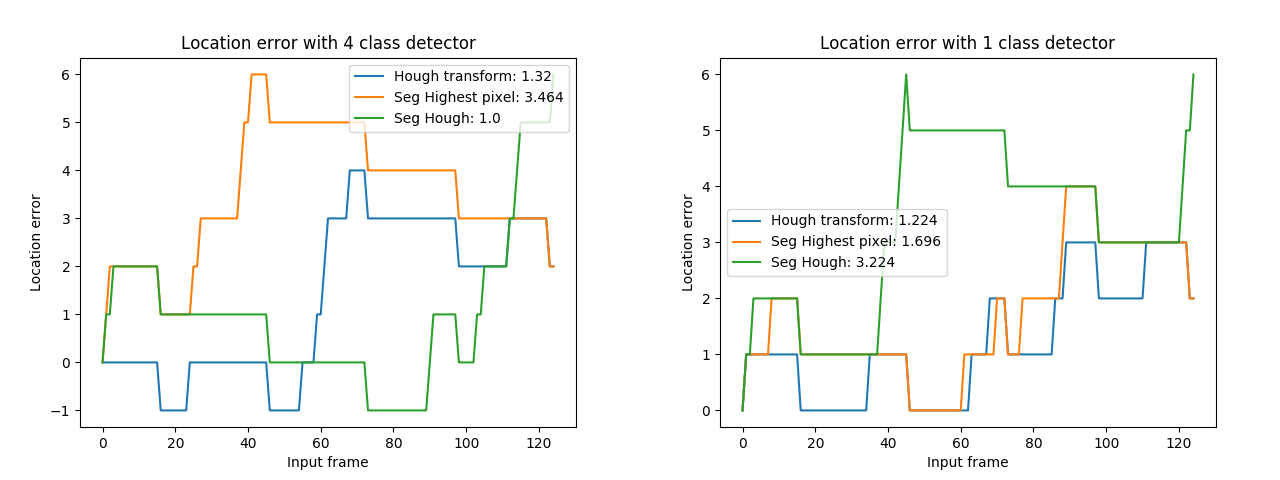
\includegraphics[width=\linewidth]{graphics/loc_acc.png}
	\end{figure}
\end{frame}

\begin{frame}[fragile]{Lokalisatie}
	\begin{itemize}
		\item Algoritme wil te snel gaan
		\item Keuze objectdetector be\"{i}nvloedt nauwkeurigheid
		\item Keuze perspectiefpuntdetector be\"{i}nvloedt nauwkeurigheid
		\item Resultaten niet accuraat omdat semantische kaart opgesteld is op basis van schattingen uit het beeldmateriaal
		\item Geen exacte gegevens beschikbaar
	\end{itemize}

	\begin{figure}
		\centering
		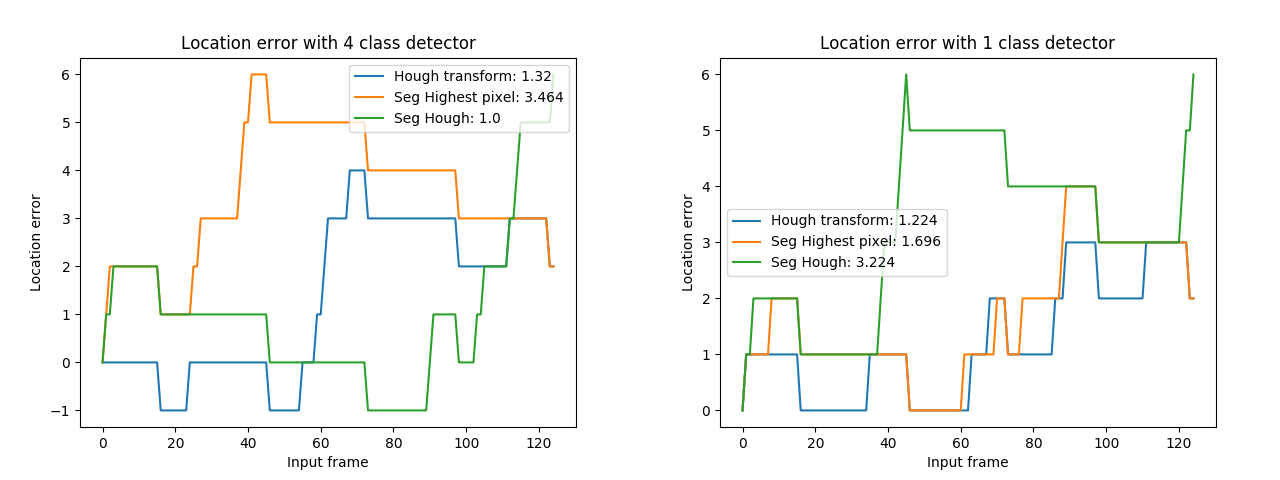
\includegraphics[width=0.8\linewidth]{graphics/loc_acc.png}
	\end{figure}
\end{frame}


\section{Demo}
\begin{frame}[fragile]{Demo}
	\begin{figure}
		\centering
		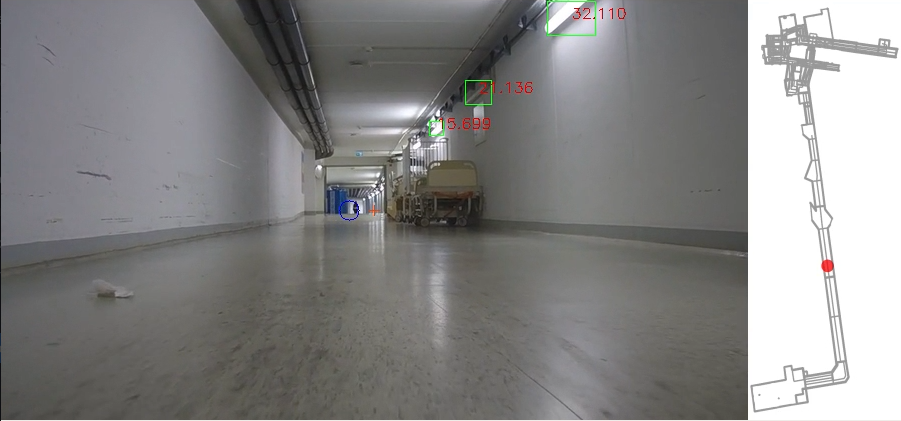
\includegraphics[width=\linewidth]{graphics/result.png}
	\end{figure}
\end{frame}

%%
%%  SECTION 4 - Besluit
%%
\section{Besluit}
\begin{frame}[fragile]{Besluit}
	\begin{itemize}
		\item Doel: Positie traking van een mobiele robot op basis van RGB camera en semantische kaart
		\item Vergelijking van verschillende detectietechnieken
		\item Opstellen en implementatie van pipeline en algoritme
		\item Resultaten van lokalisatie minder nauwkeurig door gebrek aan data
		\item YOLO object detector is mits genoeg training zeker bruikbaar in deze toepassing
		\item Door finetuning en combinatie van perspectiefpuntdetectie methoden kunnen deze ook toegepast worden
		\item Toekomstig werk
		\begin{itemize}
			\item Andere bibliotheek gebruiken voor visualisatie van de kaart om geheel te versnellen
			\item Op basis van echte gegevens de nauwkeurigheid opnieuw bepalen
		\end{itemize}
	\end{itemize}
\end{frame}

\begin{frame}[c,plain,noframenumbering]
	\begin{tikzpicture}[remember picture,overlay]
	\fill[fill=kul-blue]
		(current page.south east)  rectangle  ([shift={(0,-0.1\paperheight)}]current page.north west)   ;
	\end{tikzpicture}
	
	\centering
	\textcolor{white}{Vragen?}
	\end{frame}
\end{document}